\documentclass[11pt,letterpaper]{article}
\usepackage[utf8]{inputenc}
\usepackage[T1]{fontenc}
\usepackage{lmodern}
\usepackage[spanish,es-noshorthands]{babel}
\usepackage[margin=2.5cm]{geometry}
\usepackage{amsmath,amssymb}
\usepackage{listings}
\usepackage{graphicx}
\usepackage{xcolor}
\usepackage{enumitem}
\usepackage{url}
\usepackage[hidelinks]{hyperref}

\newcommand{\completar}[1]{\colorbox{yellow!45}{\textbf{[COMPLETAR: #1]}}}
\newcommand{\hoare}[3]{\{#1\}\ #2\ \{#3\}}

\lstset{
  language=C,
  basicstyle=\ttfamily\small,
  frame=single,
  numbers=left, numberstyle=\tiny, xleftmargin=2em,
  breaklines=true, columns=fullflexible, keepspaces=true,
  literate={á}{{\'a}}1 {é}{{\'e}}1 {í}{{\'i}}1 {ó}{{\'o}}1 {ú}{{\'u}}1 {ñ}{{\~n}}1 {—}{{-}}1
}
\lstdefinestyle{salida}{language={},numbers=none,xleftmargin=0pt,basicstyle=\ttfamily\footnotesize}

\setlist{nosep}
\setlength{\emergencystretch}{3em}

\title{Taller: Verificación formal con Frama-C}
\author{Juan Pablo Isaza Alzate (ID 1000344825)\\
David Rodríguez De La Rosa (ID 1000411459)\\[0.3cm]
Teoría de la Computación (Clase 4357) -- Grupo 7\\
Universidad EAFIT}
\date{Noviembre 2026}

\begin{document}
\maketitle

\section{Herramienta que usamos}

Usamos \textbf{Frama-C} con el plugin \textbf{WP}, que fue la que recomendaron en el enunciado. WP está basado en la lógica de Hoare: uno escribe la precondición, la postcondición y el invariante del ciclo como comentarios especiales en el código (en un lenguaje que se llama ACSL), y la herramienta calcula la precondición más débil y genera las ``obligaciones de prueba''. Esas obligaciones las resuelve un simplificador interno (Qed) o un demostrador automático como Alt-Ergo o Z3.

Lo que hace cada anotación, comparado con lo de clase:
\begin{itemize}
\item \texttt{requires} es la precondición $P$ y \texttt{ensures} es la postcondición $Q$ de la terna $\hoare{P}{C}{Q}$. En \texttt{ensures}, \texttt{\textbackslash result} es lo que retorna la función.
\item \texttt{loop invariant} es el invariante $I$ del ciclo. Frama-C revisa que se cumpla antes de entrar (lo llama \textit{established}) y que se mantenga en cada vuelta (\textit{preserved}).
\item \texttt{loop assigns} dice qué variables cambia el ciclo, para que la herramienta sepa que las demás (como \texttt{n}) no cambian.
\item \texttt{assigns \textbackslash nothing} dice que la función no modifica nada por fuera de sus variables locales.
\item \texttt{loop variant} es una expresión entera que nunca es negativa y baja en cada vuelta. Solo hace falta para la corrección total (que el ciclo termine).
\end{itemize}

\section{El programa}

Escogimos un programa que calcula $n^2$ sumando los $n$ primeros impares, porque se parece a los ejemplos de sumatorias de clase. La idea es que $1 + 3 + 5 + \dots + (2n-1) = n^2$. Por ejemplo $1+3+5+7 = 16 = 4^2$.

Tiene un ciclo y 6 asignaciones:

\begin{center}
\begin{tabular}{|c|l|l|}
\hline
\# & Asignación & Para qué sirve \\
\hline
1 & \texttt{i = 0} & cuenta cuántos impares llevamos \\
2 & \texttt{s = 0} & guarda la suma \\
3 & \texttt{impar = 1} & el primer impar \\
4 & \texttt{s = s + impar} & suma el impar que toca \\
5 & \texttt{impar = impar + 2} & pasa al siguiente impar \\
6 & \texttt{i = i + 1} & avanza el contador \\
\hline
\end{tabular}
\end{center}

Las tres primeras van antes del ciclo y las otras tres adentro. Por ejemplo, con $n = 4$ en cada vuelta $s$ va tomando los valores $0, 1, 4, 9, 16$ e \texttt{impar} los valores $1, 3, 5, 7, 9$, así que al final $s = 16 = 4^2$.

\section{Especificación}

Este es el código con las anotaciones (archivo \texttt{src/cuadrado.c}):

\begin{center}
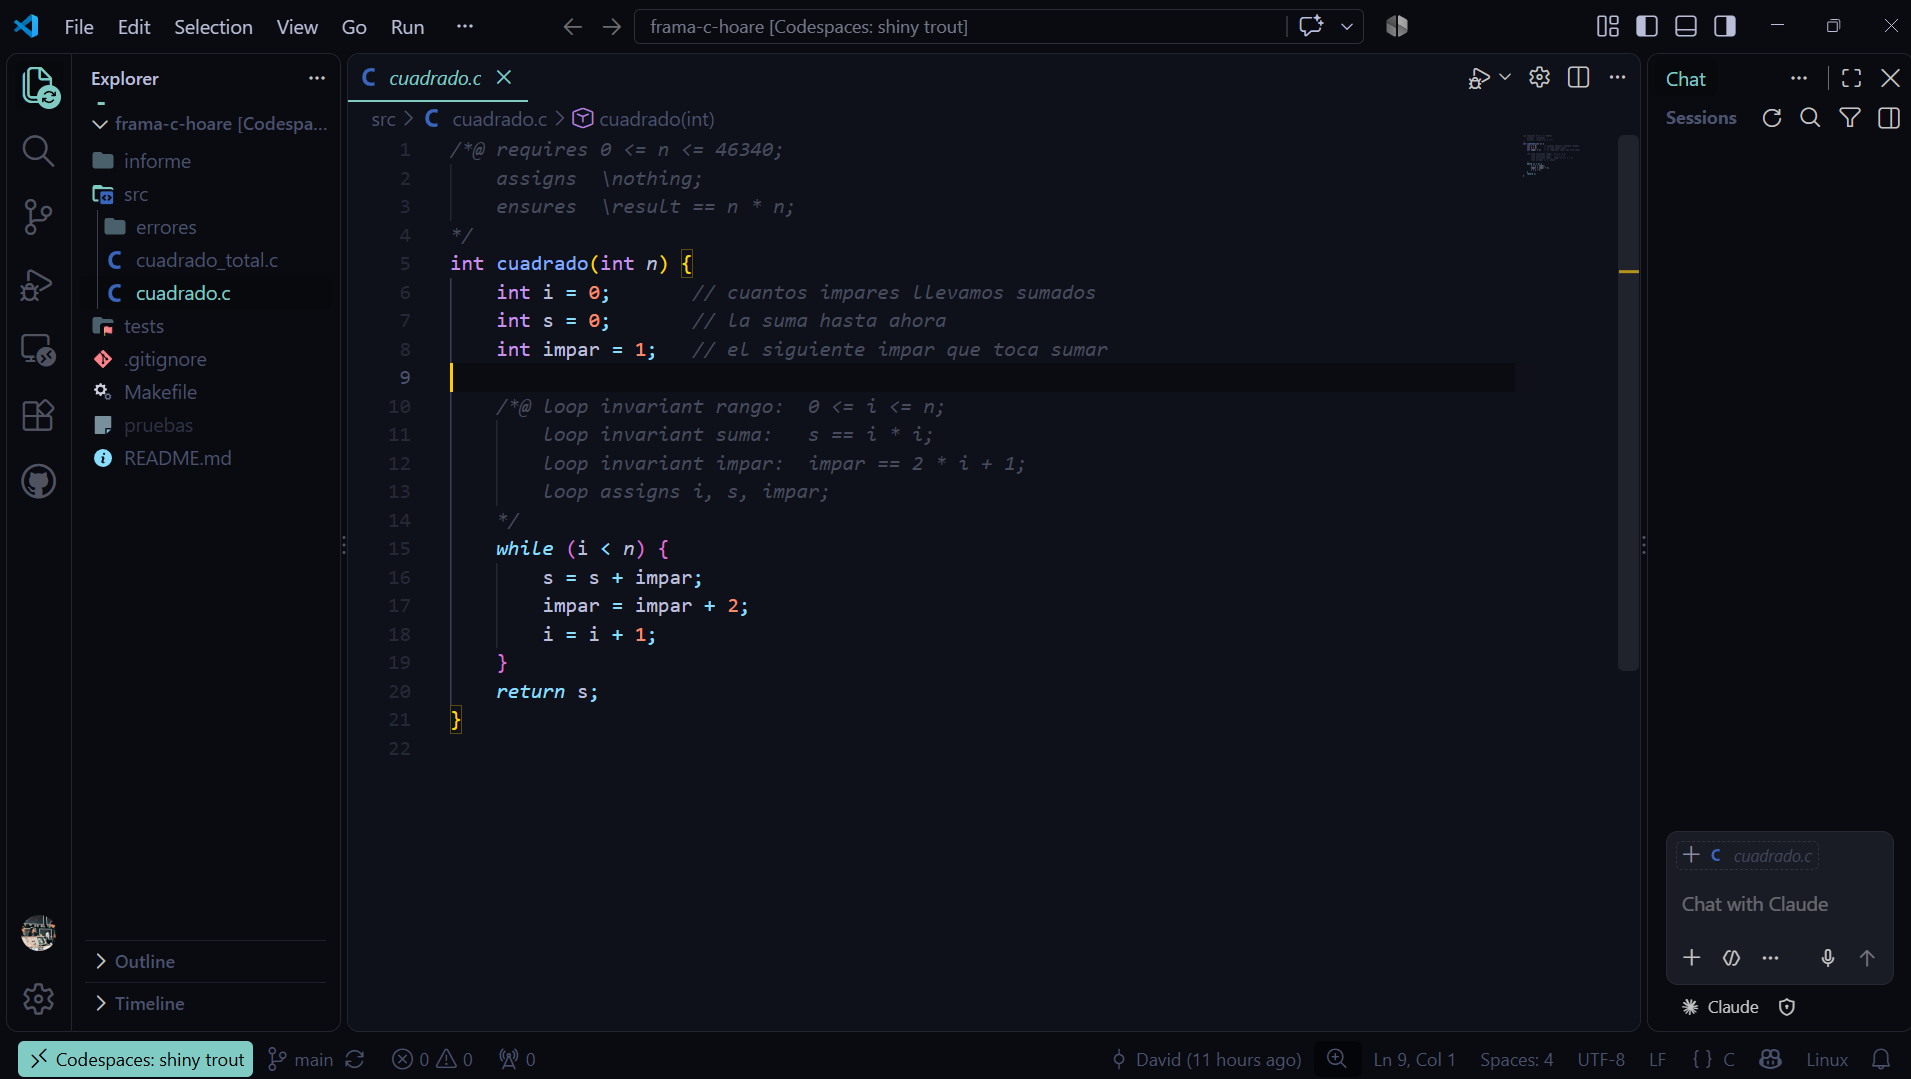
\includegraphics[width=\textwidth]{img/cuadrado_vscode.png}
\end{center}

\begin{itemize}
\item \textbf{Precondición:} $0 \le n \le 46340$. Pusimos el 46340 porque es la raíz de $2^{31}-1$ redondeada hacia abajo; si $n$ es más grande, $n^2$ ya no cabe en un \texttt{int} y se desborda.
\item \textbf{Postcondición:} el resultado es $n \cdot n$.
\item \textbf{Invariante:} $0 \le i \le n \;\wedge\; s = i^2 \;\wedge\; \mathit{impar} = 2i+1$. La parte de \texttt{impar} es necesaria: sin ella no se puede probar que $s = i^2$ se mantiene (lo probamos quitándola y la herramienta no lo pudo demostrar, ver sección~5).
\end{itemize}

\subsection*{Prueba a mano con lógica de Hoare}

Usamos las reglas vistas en clase. Las que necesitamos son la de asignación, la de concatenación y la regla while:
\[
\textbf{Asignación}\quad
\frac{}{\{Q[x \mapsto E]\}\ x := E\ \{Q\}}
\qquad\qquad
\textbf{Concatenación}\quad
\frac{\{P\}\ C_1\ \{Q\} \qquad \{Q\}\ C_2\ \{R\}}{\{P\}\ C_1; C_2\ \{R\}}
\]
\[
\textbf{Regla while}\quad
\frac{\{D \wedge I\}\ C\ \{I\}}{\{I\}\ \textcolor{blue}{\mathit{while}}\ D\ \textcolor{blue}{\mathit{do}}\ C\ \{\neg D \wedge I\}}
\]
La de asignación dice que para que $Q$ se cumpla después de $x := E$, antes se tiene que cumplir $Q$ cambiando $x$ por $E$. La de concatenación es la que deja unir la parte de antes del ciclo con el ciclo. La regla while dice que si el cuerpo mantiene el invariante cuando la condición $D$ es verdadera, al salir del ciclo se cumple $\neg D \wedge I$. En nuestro caso la condición es $D \equiv i < n$.

Para ver que el invariante sirve hay que probar tres cosas:

\textbf{1. Se cumple al inicio.} Aplicando la regla de asignación desde atrás con $i:=0$, $s:=0$, $\mathit{impar}:=1$, el invariante queda $0 \le 0 \le n \wedge 0 = 0 \wedge 1 = 1$, o sea $0 \le n$, que sale de la precondición.

\textbf{2. Se mantiene en cada vuelta.} Calculando la precondición más débil del cuerpo (de abajo hacia arriba) queda:
\[
0 \le i+1 \le n \;\wedge\; s + \mathit{impar} = (i+1)^2 \;\wedge\; \mathit{impar} + 2 = 2i+3
\]
Y si suponemos el invariante y la condición $D$ ($i < n$): $i+1 \le n$ porque $i<n$; $s + \mathit{impar} = i^2 + 2i + 1 = (i+1)^2$; y $\mathit{impar} + 2 = 2i+3$. Entonces sí se cumple.

\textbf{3. Al salir da el resultado.} Al salir tenemos $i \le n$ (invariante) y $i \ge n$ (no se cumple $D$), entonces $i = n$ y $s = n^2$. Se retorna $s$, así que el resultado es $n^2$.

Con eso queda la corrección parcial. (Si además se quiere la total, el ciclo termina porque $n - i$ es $\ge 0$ y baja de a 1 en cada vuelta.)

\section{Resultados en Frama-C}

Corrimos \texttt{make verificar DOCKER=1} desde VS Code conectado a Codespace de GitHub (Frama-C 32.1 con Alt-Ergo) y esto fue lo que salió:

\begin{center}
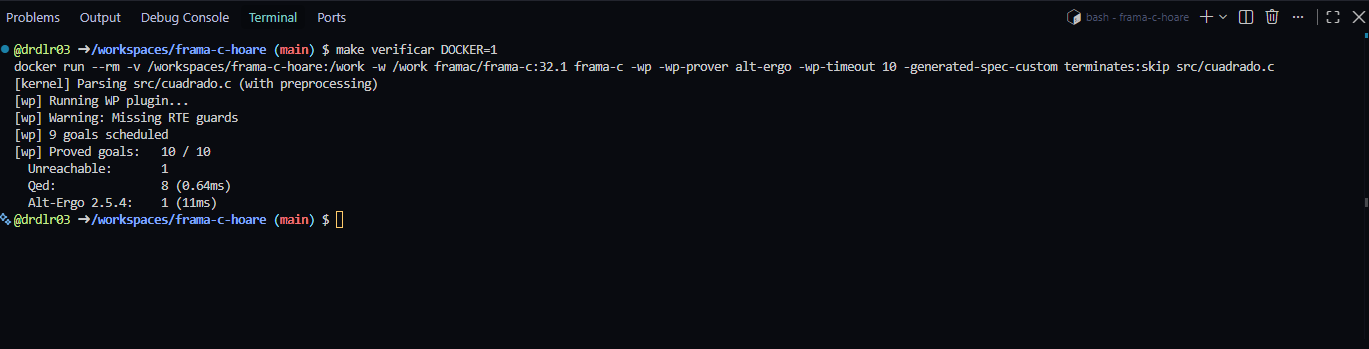
\includegraphics[width=\textwidth]{img/frama_verificar.png}
\end{center}

Todas las metas quedaron probadas (\textbf{10/10}), o sea que el programa es parcialmente correcto. Las 10 se reparten así:
\begin{itemize}
\item \textbf{8} las resolvió Qed (el simplificador de Frama-C) sin ayuda.
\item \textbf{1} la resolvió Alt-Ergo: \texttt{suma\_preserved}, porque tiene la multiplicación $i \cdot i$.
\item \textbf{1} sale como \texttt{Unreachable}: es la meta de \texttt{exits} (que la función no termina el programa con \texttt{exit}). Frama-C ve de una que el código nunca llama a \texttt{exit}, así que la da por probada sin mandarla a ningún demostrador. Por eso dice \texttt{9 goals scheduled} pero al final cuenta 10.
\end{itemize}

Cada meta que genera Frama-C corresponde a una parte de la prueba a mano:

\begin{center}
\begin{tabular}{|l|l|}
\hline
Meta (todas empiezan por \texttt{typed\_cuadrado\_}) & Qué revisa \\
\hline
\texttt{loop\_invariant\_rango\_established} & punto 1, para $0 \le i \le n$ \\
\texttt{loop\_invariant\_suma\_established} & punto 1, para $s = i^2$ \\
\texttt{loop\_invariant\_impar\_established} & punto 1, para $\mathit{impar} = 2i+1$ \\
\texttt{loop\_invariant\_rango\_preserved} & punto 2, para $0 \le i \le n$ \\
\texttt{loop\_invariant\_suma\_preserved} & punto 2, para $s = i^2$ (la de Alt-Ergo) \\
\texttt{loop\_invariant\_impar\_preserved} & punto 2, para $\mathit{impar} = 2i+1$ \\
\texttt{ensures} & punto 3, el resultado es $n^2$ \\
\texttt{loop\_assigns} & el ciclo solo cambia $i$, $s$ e \texttt{impar} \\
\texttt{assigns} & la función no cambia nada por fuera \\
\texttt{exits} & la función no se sale con \texttt{exit} (\texttt{Unreachable}) \\
\hline
\end{tabular}
\end{center}

El \texttt{Warning: Missing RTE guards} es porque en esta corrida no le pedimos revisar desbordamientos. Con \texttt{make verificar-total DOCKER=1}, que usa \texttt{-wp-rte} para revisar desbordamientos y además tiene el \texttt{loop variant n - i} (archivo \texttt{src/cuadrado\_total.c}), salieron \textbf{17/17}: ahí también queda probado que el ciclo termina (la captura está en la sección 6).

Al principio la parcial en Frama-C 32 nos dio 10/11 y no entendíamos por qué. Lo que pasa es que desde la versión 27 Frama-C le agrega solo a cada función dos metas más: la de \texttt{exits} y una de \texttt{terminates}, que pide probar que el ciclo termina. Esa segunda ya es corrección total, entonces sin el \texttt{loop variant} no se puede probar y sale \texttt{Timeout}. Para la parcial la quitamos con la opción \texttt{-generated-spec-custom terminates:skip} (el Makefile ya la pone) y en la total sí se prueba gracias al variante.

\section{Probando con errores}

Para ver que la herramienta de verdad detecta errores, hicimos dos versiones malas (carpeta \texttt{src/errores/}):
\begin{itemize}
\item Quitando el invariante de \texttt{impar}: queda \textbf{7/8}, falla \texttt{suma\_preserved} con \texttt{Timeout}. Sin ese invariante Frama-C no sabe cuánto vale \texttt{impar}, entonces no puede probar que $s + \mathit{impar} = (i+1)^2$.
\item Quitando el $n \le 46340$ y usando \texttt{-wp-rte}: queda \textbf{13/14}, falla \texttt{assert\_rte\_signed\_overflow\_2}, porque con $n$ grande \texttt{s + impar} se podría desbordar.
\end{itemize}
Con esto se ve que tanto el invariante de \texttt{impar} como la cota de la precondición sí hacen falta. Esto se corre con \texttt{make errores DOCKER=1}.

\section{Cómo ejecutarlo}

Se corre desde un Codespace de GitHub, así que no hay que instalar nada en el computador. Hay dos formas de abrirlo:

\begin{itemize}
\item \textbf{Desde el navegador:} en la página del repositorio se le da a \textit{Code $\to$ Codespaces $\to$ Create codespace on main}. Eso abre un VS Code en el navegador.
\item \textbf{Desde VS Code (lo que hicimos nosotros):} se instala la extensión \textit{GitHub Codespaces}, se abre la paleta con \texttt{Ctrl+Shift+P}, se escribe \textit{Codespaces: Connect to Codespace} y se escoge el Codespace. La terminal de VS Code queda corriendo en el Codespace.
\end{itemize}

El Codespace ya trae Docker, y con \texttt{DOCKER=1} el Makefile usa la imagen oficial de Frama-C. La primera vez se demora unos minutos descargándola.

Los comandos son \texttt{make verificar DOCKER=1} (corrección parcial), \texttt{make verificar-total DOCKER=1} (corrección total), \texttt{make errores DOCKER=1} (las versiones malas, que tienen que fallar) y \texttt{make pruebas} (pruebas normales con gcc). Así nos quedó a nosotros la corrección total y las pruebas, corriéndolo desde VS Code conectado al Codespace:

\begin{center}
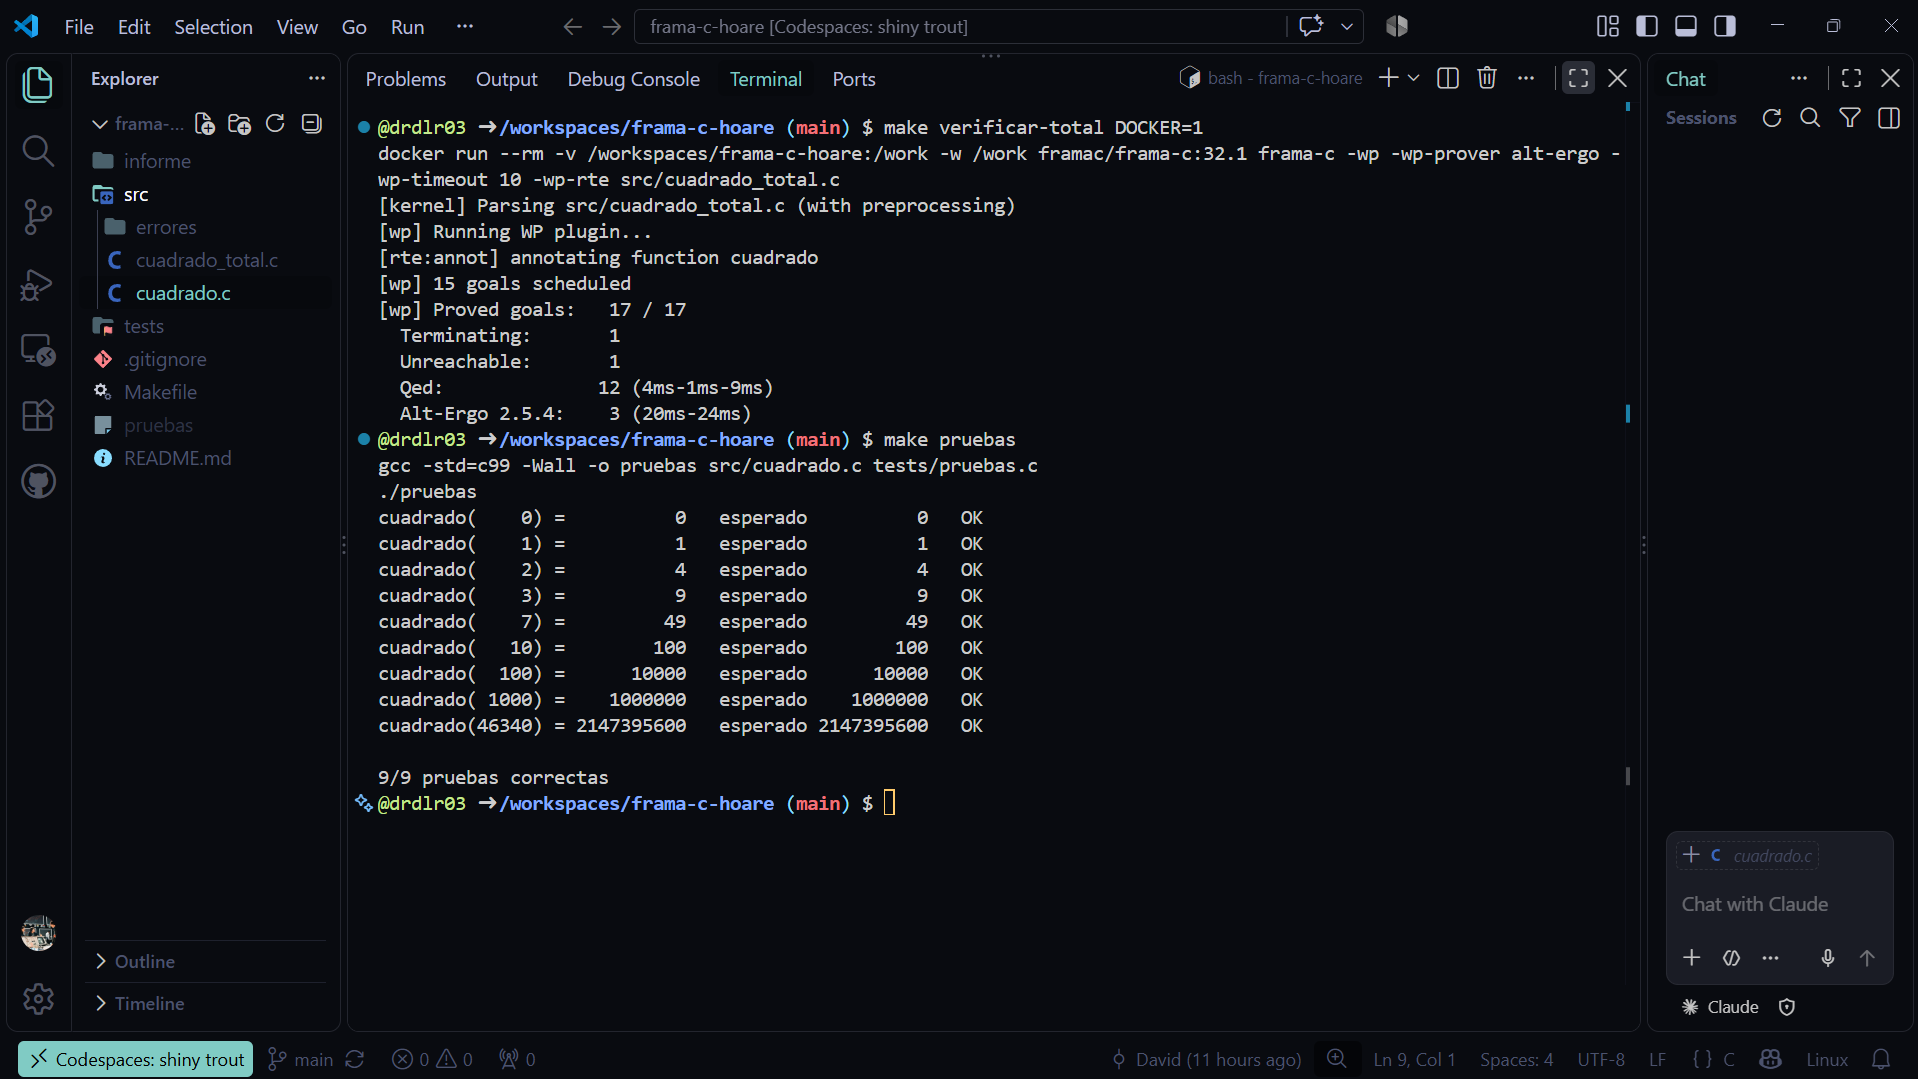
\includegraphics[width=\textwidth]{img/ejecucion_codespaces.png}
\end{center}

\section{Sistema operativo y versiones}

\begin{center}
\begin{tabular}{|l|l|}
\hline
Qué & Versión / detalle \\
\hline
Nuestro computador & Windows 11 con VS Code \\
Dónde corre Frama-C & GitHub Codespaces (por dentro es Linux) \\
Frama-C (con el plugin WP) & 32.1, imagen de Docker \texttt{framac/frama-c:32.1} \\
Demostrador automático & Alt-Ergo 2.5.4 (viene en la imagen) \\
Pruebas normales & gcc del Codespace \\
\hline
\end{tabular}
\end{center}

Frama-C no funciona directamente en Windows, solo en Linux o macOS. Por eso lo corrimos en un Codespace, que es una máquina en la nube de GitHub; así no tuvimos que instalar nada en nuestros computadores. Como usamos la imagen oficial de Docker, cualquiera que lo corra con \texttt{DOCKER=1} obtiene exactamente las mismas versiones que nosotros.

Así se reparte el trabajo entre las partes: Frama-C lee el código en C con las anotaciones ACSL, el plugin WP calcula la precondición más débil y arma las metas, Qed (que viene dentro de WP) resuelve las fáciles, y las que tienen cosas más difíciles, como la multiplicación $i \cdot i$, se las pasa a Alt-Ergo.

\section{Repositorio}

El código, las salidas de Frama-C y este informe están en: \url{https://github.com/drdlr03/frama-c-hoare}

\section{Uso de inteligencia artificial}

\textbf{Herramienta utilizada:} Claude Opus 5.5 y Claude Code.

\subsection*{Trabajo realizado por el equipo}

Una de las partes en las que más trabajamos fue en entender cómo funcionaba la verificación formal. Revisamos paso a paso la prueba a mano con lógica de Hoare de la sección 3, tratando de comprender cómo se relacionan las precondiciones, las instrucciones del programa y las postcondiciones. También estudiamos cómo se obtiene la precondición más débil del cuerpo del ciclo y por qué, al finalizar, el invariante junto con la condición de salida permite demostrar que $s = n^2$.

Además, trabajamos en entender la parte matemática del algoritmo. Vimos que en cada iteración se suma un número impar ($2i+1$) y que, gracias a la igualdad $i^2 + (2i+1) = (i+1)^2$, la suma de los primeros $n$ números impares permite obtener el cuadrado de $n$.

También revisamos las anotaciones ACSL y la función que cumple cada una. Entendimos que el invariante $s = i^2$ necesita complementarse con $\mathit{impar} = 2i+1$ para demostrar que se mantiene durante las iteraciones. De igual forma, revisamos por qué se utiliza la restricción $n \leq 46340$ para evitar el desbordamiento de los enteros y para qué sirve el \texttt{loop variant} $n-i$ al demostrar que el ciclo termina.

Por otra parte, ejecutamos las verificaciones en GitHub Codespaces y revisamos los resultados que nos daba Frama-C. No nos quedamos solamente con ver si las pruebas salían bien o mal, sino que buscamos entender qué significaba cada resultado y por qué algunas condiciones se verificaban y otras no. También analizamos las versiones del programa que tenían errores y revisamos por qué no pasaban la verificación. Finalmente, trabajamos en la organización del repositorio, la revisión de los archivos y la compilación del informe.

\subsection*{Apoyo de la inteligencia artificial}

Durante el proyecto utilizamos Claude y Claude Code como apoyo en algunas partes del desarrollo. Principalmente, nos ayudó con una primera versión del código en C y las anotaciones ACSL, además de proponer algunas modificaciones y ejemplos para comprobar el funcionamiento del programa.

También nos ayudó a resolver algunas dudas técnicas al trabajar con Frama-C, especialmente con los comandos necesarios para ejecutar las verificaciones desde la terminal de VS Code conectada a GitHub Codespaces. Por último, nos sirvió como apoyo para organizar y corregir algunos aspectos del informe.

Sin embargo, no nos limitamos a usar lo que nos daba la IA: a partir de eso fuimos revisando el código, ejecutando las verificaciones, estudiando las demostraciones y analizando los resultados, para entender cómo funcionaba el proyecto y qué era lo que estábamos verificando.

\section*{Referencias}
\begin{enumerate}[label={[\arabic*]}]
\item A. Blanchard. \emph{Introduction to C program proof with Frama-C and its WP plugin}. \url{https://allan-blanchard.fr/frama-c-wp-tutorial.html}
\item Frama-C. \url{https://frama-c.com}
\item P. Baudin et al. \emph{ACSL: ANSI/ISO C Specification Language}. \url{https://frama-c.com/html/acsl.html}
\item W. K. Grassmann y J.-P. Tremblay. \emph{Logic and Discrete Mathematics: A Computer Science Perspective}. Prentice Hall, 1996.
\end{enumerate}

\end{document}
